\chapter{HASIL DAN PEMBAHASAN}

Setelah dilakukan penjelasan terhadap langkah-langkah mulai dari pengumpulan data, \textit{data preprocessing}, Pembuatan dan Pelatihan Model, dan Pengujian Model. Selanjutnya, menampilkan hasil dari tahapan-tahapan tersebut. Kinerja model klasifikasi dalam melakukan pengklasifikasian juga akan diperlihatkan untuk mengukur seberapa baik model tersebut dalam mengklasifikasikan citra makanan. \textit{Confussion matrix} dan \textit{classification report} akan digunakan sebagai alat ukur untuk evaluasi pada klasifikasi citra makanan tersebut. Semakin tinggi akurasi klasifikasi berarti performa klasifikasi juga semakin baik.

\section{Hasil Pengumpulan Data}
Hasil pengumpulan data citra makanan yang diperoleh menggunakan teknik \textit{Scraping} berjumlah sebanyak 5000 citra makanan yang terbagi dalam 10 kelas (ayam bakar, bakso, gado gado, gudeg, nasi goreng, pempek, rawon, rendang, sate, dan soto), dimana setiap kelas memiliki total 500 citra makanan.

\begin{afigure}
    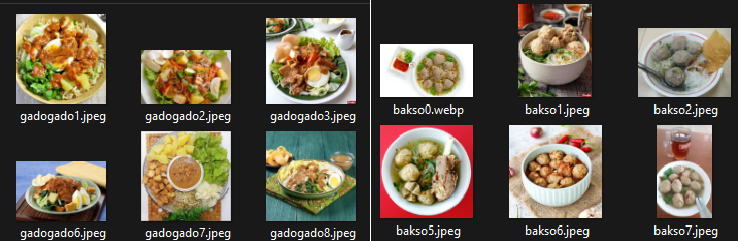
\includegraphics[width=0.95\textwidth, center]{images/citra-makanan.png}
    \caption{Hasil pengumpulan data citra makanan}
    \label{fig:citra-makanan}
\end{afigure}

Gambar 4.1 merupakan contoh data citra makanan yang berhasil dikumpulkan menggunakan teknik \textit{scraping} dalam penelitian ini. Gambar 4.1 menunjukan perbedaan signifikan dari gado-gado dan bakso. Perbedaan signifikan tersebut meliputi bentuk dan warna.

\section{Hasil \textit{Data Preprocessing}}
Hasil dari \textit{data preprocessing} terbagi menjadi menjadi 4 bagian, yaitu:
\begin{enumerate}
    \item Hasil \textit{Data Cleaning}.
    \item Hasil \textit{Undersampling}.
    \item Hasil \textit{Split Data}.
    \item Hasil \textit{Data Normalization} dan \textit{Data Augmentation}.
\end{enumerate}

\subsection{Hasil \textit{Data Cleaning}}
Setelah data berhasil dikumpulkan menggunakan teknik \textit{scraping}, kemudian dilakukan proses \textit{Data Cleaning}. Tahap ini akan memperlihatkan hasil dari \textit{data cleaning}. Berikut hasil dari \textit{data cleaning} pada Tabel 4.1

\begin{atable}
    \centering
    \caption{Hasil Cleaning Data}
    \label{table:hasil-cleaning}
    \csvreader[
        head to column names,
        separator=semicolon,
        tabular={|c|c|},
        table head=\hline
            \rowcolor{gray!50!black}
            \color{white} Makanan & 
            \color{white} Jumlah Data \\ \hline,
        late after line=\\ \hline,
        late after last line=\\ \hline
        ]
        {tables/cleaning.csv}
        {makanan=\makanan, jumlah=\jumlah}
        {\makanan & \jumlah}
\end{atable}

Hal ini dilakukan karena data citra yang didapatkan dari \textit{scraping} banyak yang \textit{duplicate} dan banyak citra yang tidak sesuai dengan makanan yang dimaksud. \textit{Data Cleaning} dilakukan agar dapat memastikan konsistensi data dan model dapat mengenali data yang benar.

\subsection{Hasil \textit{Undersampling}}
Setelah melakukan \textit{data cleaning}, langkah berikutnya adalah \textit{Undersampling} pada data. \textit{Undersampling} dilakukan untuk menangani ketidakseimbangan data yang ada dalam dataset. Ketidakseimbangan data terjadi ketika jumlah citra dalam satu kelas makanan jauh lebih banyak dibandingkan dengan kelas lainnya. Hasil \textit{Undersampling} dapat dilihat pada Tabel 4.2.

\begin{atable}
    \centering
    \caption{Hasil Undersampling}
    \label{table:hasil-undersampling}
    \csvreader[
        head to column names,
        separator=semicolon,
        tabular={|c|c|c|},
        table head=\hline
            \rowcolor{gray!50!black}
            \color{white} Makanan & 
            \color{white} Jumlah Sebelum Undersampling &
            \color{white} Jumlah Sesudah Undersampling \\ \hline,
        late after line=\\ \hline,
        late after last line=\\ \hline
        ]
        {tables/undersampling.csv}
        {makanan=\makanan, sebelum=\sebelum, sesudah=\sesudah}
        {\makanan & \sebelum & \sesudah}
\end{atable}

Setelah dilakukan \textit{Undersampling}, semua data pada tiap kelas menjadi 200 citra. \textit{Undersampling} dilakukan untuk mengurangi adanya bias. Bias biasa terjadi ketika terjadi ketidakseimbangan data.

\subsection{Hasil \textit{Split Data}}
Setelah dilakukan proses \textit{Undersampling}, data kemudian dibagi menjadi menjadi data latih dan data uji. Berikut hasil \textit{Split Data} pada Gambar 4.2.

\begin{afigure}
    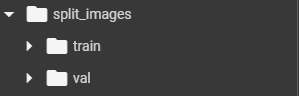
\includegraphics[width=0.5\textwidth, center]{images/hasil-split.png}
    \caption{Hasil Split Data}
    \label{fig:hasil-split}
\end{afigure}
Setelah dilakukan \textit{Split Data}, dataset sekarang mempunyai 2 bagian, yaitu data latih dan data uji. Dengan rasio 80\% untuk data latih, dan 20\% untuk data uji, data latih mempunyai 160 citra tiap kelasnya, sedangkan data uji mempunyai 40 citra tiap kelasnya.

\subsection{Hasil \textit{Data Normalization} dan \textit{Data Augmentation}}
Setelah dilakukan \textit{Split Data} menjadi data uji dan data latih, kemudian dilakukan proses \textit{Data Normalization} dan \textit{Data Augmentation}. Berikut contoh dataset sebelum dilakukan proses \textit{Data Normalization} dan \textit{Data Augmentation} pada Gambar 4.3.

\begin{afigure}
    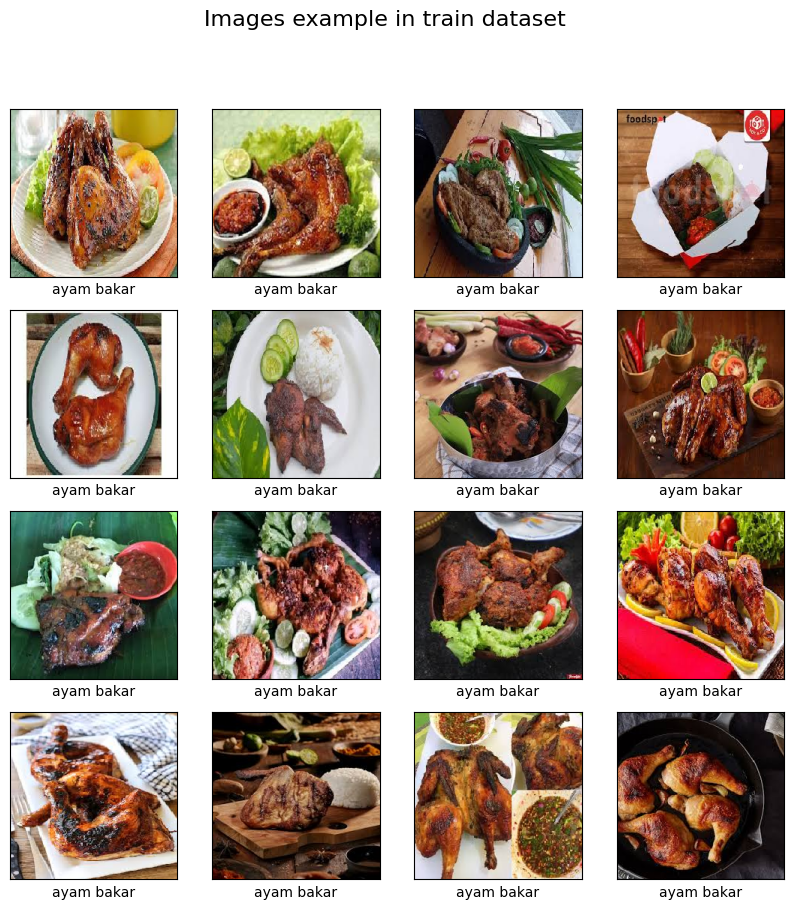
\includegraphics[height=0.6\textheight, width=0.9\textwidth, center]{images/raw-dataset.png}
    \caption{Data Sebelum Proses \textit{Data Normalization} dan \textit{Data Augmentation}}
    \label{fig:sebelum-augmentasi}
\end{afigure}

\begin{afigure}
    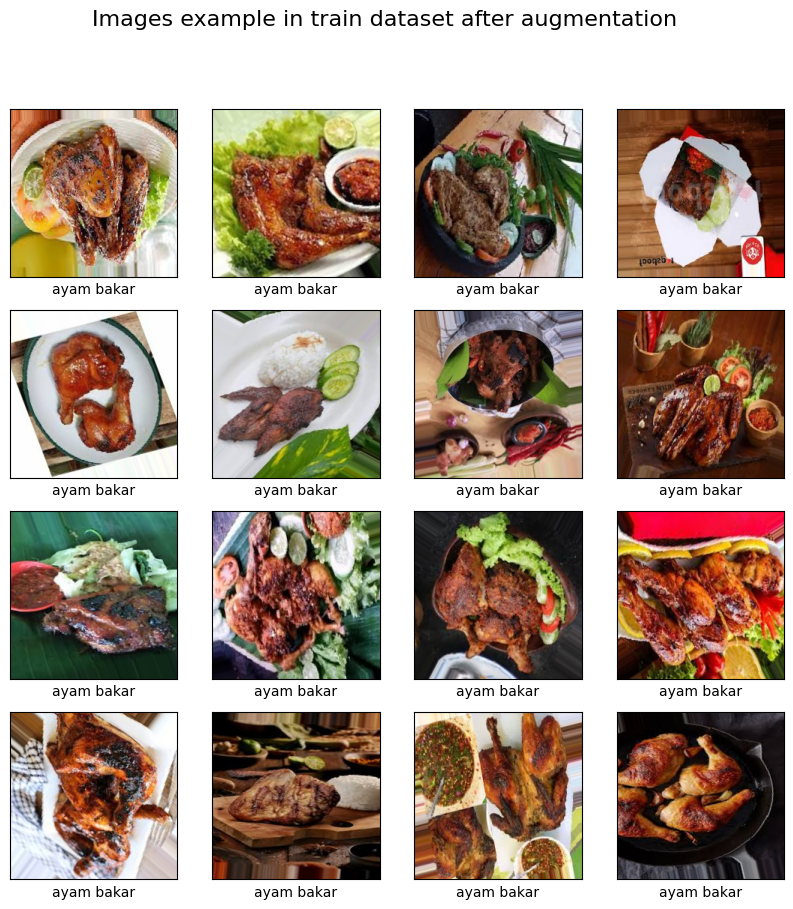
\includegraphics[height=0.6\textheight, width=0.9\textwidth, center]{images/augmented.png}
    \caption{Data Sesudah Proses \textit{Data Normalization} dan \textit{Data Augmentation}}
    \label{fig:sesudah-augmentasi}
\end{afigure}

Pada Gambar 4.4, terlihat citra yang telah dilakukan proses \textit{Data Normalization} dan \textit{Data Augmentation} terlihat berbeda dengan sebelumnya. Setelah dilakukan proses tersebut, terlihat beberapa citra terbalik secara vertikal ataupun horizontal, beberapa citra mengalami rotasi, dan beberapa citra diperbesar.

\section{Hasil Pembuatan dan Pelatihan Model}
Setelah dilakukan proses \textit{Data Preprocessing}, kemudian dilakukan proses Pembuatan dan Pelatihan Model. Hasil Pembuatan dan Pelatihan Model dibagi menjadi 2 bagian, yaitu:
\begin{enumerate}
    \item Hasil \textit{Transfer Learning} EfficientNetV2
    \item Hasil \textit{Training Model}
\end{enumerate}

\subsection{Hasil \textit{Transfer Learning} EfficientNetV2}
\begin{afigure}
    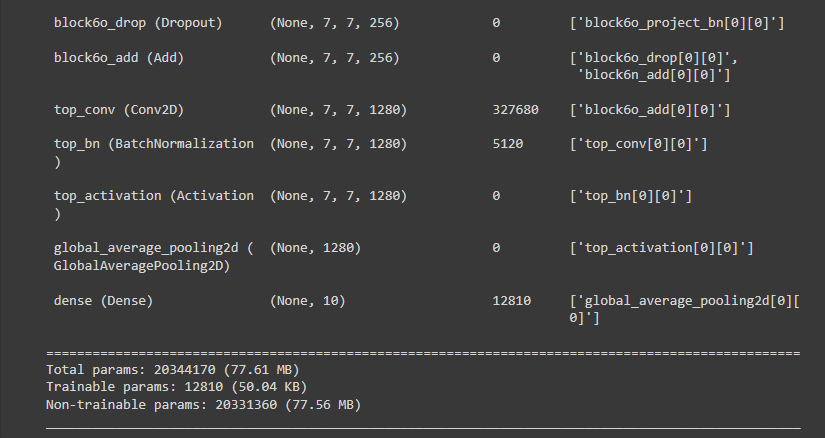
\includegraphics[width=0.9\textwidth, center]{images/model-summary.png}
    \caption{Ringkasan Model Hasil Transfer Learning EfficientNetV2}
    \label{fig:model-summary}
\end{afigure}

Gambar 4.5 merupakan ringkasan dari model yang telah dibuat. Pada penelitian ini, model yang telah dibuat menggunakan \textit{layer} dari EfficientNetV2, lalu ditambahkan lapisan tambahan yaitu lapisan GlobalAveragePooling2D dan lapisan Dense dengan aktivasi softmax. Berikut adalah penjelasan dari parameter yang terdapat dalam Gambar 4.5:

\begin{itemize}
    \item \textbf{Total params: 20,344,170 (77.61 MB)}: Ini adalah jumlah total parameter dalam model yang telah dibuat. Parameter ini mencakup semua bobot (\textit{weights}) dan bias (\textit{biases}) yang ada di dalam model, baik yang dapat dilatih maupun yang tidak dapat dilatih.
    \item \textbf{Trainable params: 12,810 (50.04 KB)}: Ini adalah jumlah parameter yang dapat dilatih dalam model yang telah dibuat. Dalam kasus ini, hanya ada 12,810 parameter yang dapat dilatih. Parameter ini berasal dari lapisan tambahan yang ditambahkan setelah model pra-latih EfficientNetV2S, yaitu lapisan GlobalAveragePooling2D dan lapisan Dense dengan aktivasi softmax.
    \item \textbf{Non-trainable params: 20,331,360 (77.56 MB)}: Ini adalah jumlah parameter yang tidak dapat dilatih. Parameter ini merupakan parameter dari model pra-latih EfficientNetV2S yang digunakan. Karena diatur pre\_trained\_model.trainable = False, parameter dalam EfficientNetV2S tidak akan diperbarui selama pelatihan.
\end{itemize}

\subsection{Hasil \textit{Training Model}}
Setelah dilakukan pembuatan model dengan menggunakan metode \textit{transfer learning}, kemudian dilakukan proses \textit{training model} atau pelatihan model. Pada penelitian ini, model dilatih menggunakan \textit{learning rate} sebesar 0.001, callback ModelCheckPoint untuk menyimpan model terbaik berdasarkan val\_loss terkecil, dan menggunakan epoch sebanyak 50 epoch. 
Hasil \textit{Training Model} dibagi menjadi 2 bagian, yaitu:
\begin{enumerate}
    \item Hasil \textit{Training Model} menggunakan Google Colab GPU T4
    \item Hasil \textit{Training Model} menggunakan mesin DGX A100 Universitas Gunadarma.
\end{enumerate}

\subsubsection{Hasil \textit{Training Model} menggunakan Google Colab GPU T4}
Berikut tabel hasil pelatihan model menggunakan Google Colab GPU T4 dengan konfigurasi tersebut:
\begin{longtable}{|c|c|c|c|c|}
    \caption{Hasil Training Model menggunakan Google Colab GPU T4} \label{table:hasil-training} \\ \hline
    \rowcolor{gray!50!black}
    \color{white} Epoch &
    \color{white} Loss & 
    \color{white} Accuracy &
    \color{white} Val Loss &
    \color{white} Val Accuracy \\ \hline
    \endfirsthead
    
    \hline
    \rowcolor{gray!50!black}
    \color{white} Epoch &
    \color{white} Loss & 
    \color{white} Accuracy &
    \color{white} Val Loss &
    \color{white} Val Accuracy \\ \hline
    \endhead
    
    \csvreader[
        head to column names,
        late after line=\\ \hline,
        late after last line=\\ \hline
        ]
        {tables/training-history.csv}
        {loss=\loss, accuracy=\accuracy, val_loss=\valloss, val_accuracy=\valaccuracy}
        {%
            \ifthenelse{\equal{\thecsvrow}{49}}{%
                \bfseries\thecsvrow & \bfseries\num{\loss} & \bfseries\num{\accuracy} & \bfseries\num{\valloss} & \bfseries\num{\valaccuracy}%
            }{%
                \thecsvrow & \num{\loss} & \num{\accuracy} & \num{\valloss} & \num{\valaccuracy}%
            }%
        }
\end{longtable}

Tabel 4.3 merupakan hasil pelatihan model menggunakan Google Colab GPU T4 sebanyak 50 epoch. Model terbaik yang diambil merupakan model dengan \textit{Val Loss} terkecil, berdasarkan hasil pelatihan model pada Tabel 4.3, model terbaik merupakan model pada Epoch ke-49, dengan \textit{Val Loss} sebesar 0.3944 dan \textit{Val Accuracy} sebesar 0.8750 atau 87.50\%. Dengan menggunakan Google Colab GPU T4, pelatihan memakan waktu selama 22 menit.

\subsubsection{Hasil \textit{Training Model} menggunakan mesin DGX A100 Universitas Gunadarma}
Berikut tabel hasil pelatihan model menggunakan mesin DGX A100 Universitas Gunadarma dengan konfigurasi tersebut:
\begin{longtable}{|c|c|c|c|c|}
    \caption{Hasil Training Model menggunakan mesin DGX A100 Universitas Gunadarma} \label{table:hasil-training-dgx} \\ \hline
    \rowcolor{gray!50!black}
    \color{white} Epoch &
    \color{white} Loss & 
    \color{white} Accuracy &
    \color{white} Val Loss &
    \color{white} Val Accuracy \\ \hline
    \endfirsthead
    
    \hline
    \rowcolor{gray!50!black}
    \color{white} Epoch &
    \color{white} Loss & 
    \color{white} Accuracy &
    \color{white} Val Loss &
    \color{white} Val Accuracy \\ \hline
    \endhead
    
    \csvreader[
        head to column names,
        late after line=\\ \hline,
        late after last line=\\ \hline
        ]
        {tables/training-history-dgx.csv}
        {loss=\loss, accuracy=\accuracy, val_loss=\valloss, val_accuracy=\valaccuracy}
        {%
            \ifthenelse{\equal{\thecsvrow}{50}}{%
                \bfseries\thecsvrow & \bfseries\num{\loss} & \bfseries\num{\accuracy} & \bfseries\num{\valloss} & \bfseries\num{\valaccuracy}%
            }{%
                \thecsvrow & \num{\loss} & \num{\accuracy} & \num{\valloss} & \num{\valaccuracy}%
            }%
        }
\end{longtable}

Tabel 4.4 merupakan hasil pelatihan model menggunakan mesin DGX A100 Universitas Gunadarma sebanyak 50 epoch. Model terbaik yang diambil merupakan model dengan \textit{Val Loss} terkecil, berdasarkan hasil pelatihan model pada Tabel 4.4, model terbaik merupakan model pada Epoch ke-50, dengan \textit{Val Loss} sebesar 0.3925 dan \textit{Val Accuracy} sebesar 0.8725 atau 87.25\%. Dengan menggunakan mesin DGX A100 Universitas Gunadarma, pelatihan memakan waktu selama 11 menit saja.

\section{Hasil Pengujian Model}
Setelah melalui tahap \textit{Training Model}, kemudian dilakukan tahap terakhir yaitu Pengujian Model. Hasil Pengujian Model dibagi menjadi 2 bagian, yaitu:
\begin{enumerate}
    \item Hasil Pengujian Model Google Colab GPU T4
    \item Hasil Pengujian Model mesin DGX A100 Universitas Gunadarma
\end{enumerate}

\subsection{Hasil Pengujian Model Google Colab GPU T4}
Hasil Pengujian Model Google Colab GPU T4 dibagi menjadi 3 bagian, yaitu:
\begin{enumerate}
    \item Hasil Evaluasi Model
    \item Hasil Visualisasi Grad-CAM
    \item Hasil Pengujian Model menggunakan data nutrisi makanan
\end{enumerate}

\subsubsection{Hasil Evaluasi Model}
Tahap pertama pada Evaluasi Model yaitu untuk mengetahui model tersebut termasuk \textit{overfit, good fit} atau \textit{underfit}. Untuk mengetahui hal tersebut, dapat dilakukan dengan membuat visualisasi dari hasil pelatihan model dengan diagram garis. Berikut hasil visualisasi pelatihan model dengan diagram garis:

\begin{afigure}
    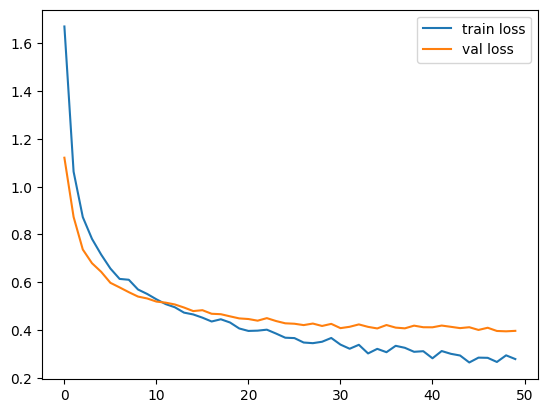
\includegraphics[height=0.4\textheight, width=0.9\textwidth, center]{images/train-loss.png}
    \label{fig:train-loss}
\end{afigure}
\pagebreak
\begin{afigure}
    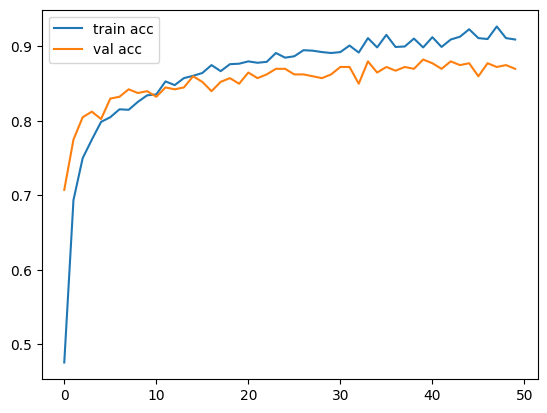
\includegraphics[height=0.4\textheight, width=0.9\textwidth, center]{images/train-acc.png}
    \caption{Visualisasi Pelatihan Model Google Colab GPU T4}
    \label{fig:train-acc}
\end{afigure}

Pada Gambar 4.6, terlihat \textit{train loss} dan \textit{val loss} mendekati satu sama lain dan terus menurun hingga datar dari beberapa titik hingga akhir. Kemudian, \textit{train acc} dan \textit{val acc} juga mendekati satu sama lain. Hal ini dapat diartikan bahwa model tersebut termasuk \textit{good fit} dan layak dipakai.

Setelah mengetahui bahwa model layak dipakai, kemudian dilakukan \textit{
Classification Report} untuk mengetahui performa model berdasarkan metriks \textit{precision}, \textit{recall}, dan \textit{F1-Score}. Berikut hasil dari \textit{Classification Report} menggunakan \textit{library} dari sklearn:

\pagebreak

\begin{afigure}
    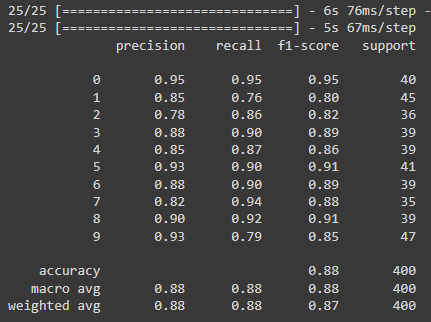
\includegraphics[width=0.9\textwidth, center]{images/classification-report.png}
    \caption{Hasil Classification Report Model Google Colab GPU T4}
    \label{fig:classification-report}
\end{afigure}


\begin{itemize}
    \item Accuracy: 0.88, menunjukkan bahwa model ini memiliki tingkat akurasi 88\% di seluruh kelas.
    \item Macro Avg: Rata-rata precision, recall, dan f1-score untuk setiap kelas, tanpa mempertimbangkan jumlah instance di setiap kelas.
    \item Weighted Avg: Rata-rata precision, recall, dan f1-score untuk setiap kelas, dengan mempertimbangkan jumlah instance di setiap kelas.
\end{itemize}

Gambar 4.7 menunjukan bahwa model memiliki performa yang baik di sebagian besar kelas, meskipun ada beberapa kelas yang memiliki nilai \textit{recall} atau \textit{precision} yang lebih rendah. Ada beberapa citra yang salah diklasifikasikan ke kelas lain, contohnya pada kelas 1 (bakso), dan kelas 9 (soto).

Setelah dilakukan \textit{Classification Report}, untuk mempermudah evaluasi model dapat menggunakan \textit{confusion matrix}. Berikut visualisasi menggunakan \textit{confusion matrix}:

\begin{afigure}
    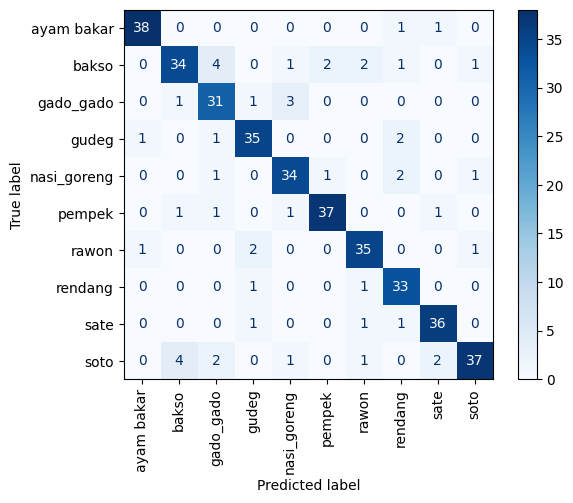
\includegraphics[width=0.9\textwidth, center]{images/confussion-matrix.png}
    \caption{Visualisasi Confusion Matrix Model Google Colab GPU T4}
    \label{fig:confussion-matrix}
\end{afigure}

Confusion matrix ini menunjukkan hasil dari model klasifikasi yang telah diuji dengan beberapa kategori makanan Indonesia. Berikut adalah interpretasi dari setiap elemen dalam \textit{confusion matrix} ini:
\begin{itemize}
    \item \textit{True label} (label sebenarnya) berada pada sumbu Y (vertikal).
    \item \textit{Predicted label} (label prediksi) berada pada sumbu X (horizontal).
\end{itemize}

Setiap sel dalam matriks menunjukkan jumlah instance yang diprediksi dalam kategori tertentu. Misalnya, sel pada baris "ayam bakar" dan kolom "ayam bakar" menunjukkan jumlah instance "ayam bakar" yang diprediksi benar oleh model. Berikut adalah beberapa poin penting yang dapat diperhatikan dari \textit{confusion matrix} pada Gambar 4.8:
\begin{itemize}
    \item \textbf{Ayam Bakar}: Dari 40 instance "ayam bakar", 38 diprediksi benar sebagai "ayam bakar", 1 diprediksi sebagai "gudeg", dan 1 diprediksi sebagai "rawon".
    \item \textbf{Bakso}: Dari 40 instance "bakso", 34 diprediksi benar sebagai "bakso", namun ada beberapa yang salah prediksi ke "gado-gado", "pempek", dan "soto".
    \item \textbf{Gado-gado}: Dari 40 instance "gado-gado", 31 diprediksi benar, namun ada beberapa yang salah prediksi ke "bakso", "gudeg", "nasi goreng", "pempek", dan "soto".
    \item \textbf{Gudeg}: Dari 40 instance "gudeg", 35 diprediksi benar, namun ada beberapa yang salah prediksi ke "gado-gado", "rawon", "rendang", dan "sate".
    \item \textbf{Nasi Goreng}: Dari 40 instance "nasi goreng", 34 diprediksi benar, namun ada beberapa yang salah prediksi ke "bakso", "gado-gado", dan "pempek", dan "soto".
    \item \textbf{Pempek}: Dari 40 instance "pempek", 37 diprediksi benar, namun ada beberapa yang salah prediksi ke "bakso" dan "nasi goreng".
    \item \textbf{Rawon}: Dari 40 instance "rawon", 35 diprediksi benar, namun ada beberapa yang salah prediksi ke "bakso", "rendang", "sate", dan "soto".
    \item \textbf{Rendang}: Dari 40 instance "rendang", 33 diprediksi benar, namun ada beberapa yang salah prediksi ke "ayam bakar", "bakso", , "gudeg", "nasi goreng", "rawon", dan "sate".
    \item \textbf{Sate}: Dari 40 instance "sate", 36 diprediksi benar, namun ada beberapa yang salah prediksi ke "ayam bakar", "pempek", dan "soto".
    \item \textbf{Soto}: Dari 40 instance "soto", 37 diprediksi benar, namun ada beberapa yang salah prediksi ke "bakso", "nasi goreng", dan "rawon".
\end{itemize}

Secara keseluruhan, model menunjukkan performa yang cukup baik dengan sebagian besar prediksi berada di diagonal utama, yang berarti banyak instance yang diklasifikasikan dengan benar. Namun, ada beberapa kesalahan prediksi yang perlu diperhatikan untuk meningkatkan akurasi model lebih lanjut.

\subsubsection{Hasil Visualisasi Grad-CAM}
Setelah melakukan proses Evaluasi Model, selanjutnya dilakukan proses Visualisasi Grad-CAM. Hal ini dilakukan untuk mengetahui bagaimana model melihat citra dan area mana yang dianggap penting oleh model dalam membuat prediksi. Berikut hasil visualisasi menggunakan Grad-CAM:

\begin{afigure}
    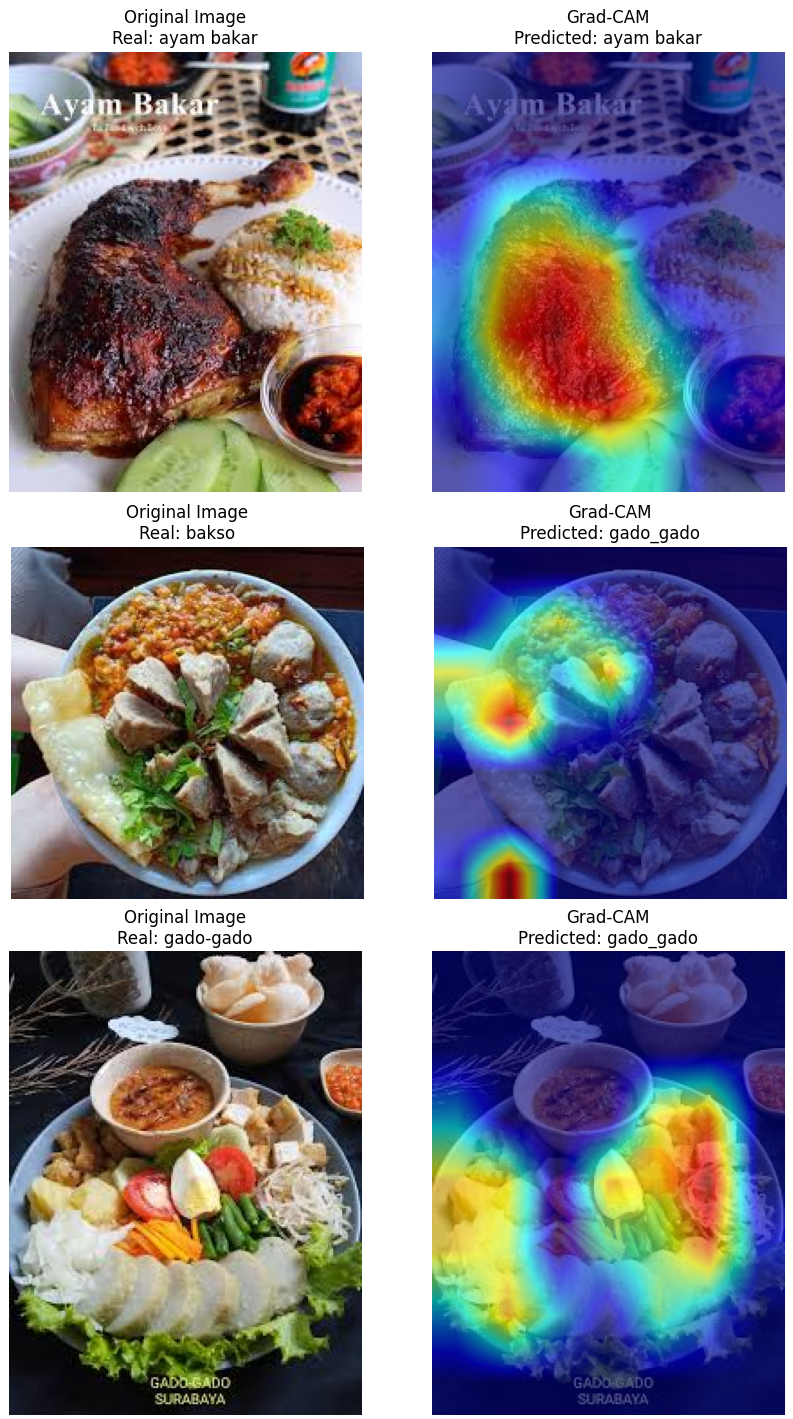
\includegraphics[height=0.75\textheight, width=0.9\textwidth, center]{images/grad-cam-1.png}
    \label{fig:grad-cam-1}
\end{afigure}
\clearpage
\begin{afigure}
    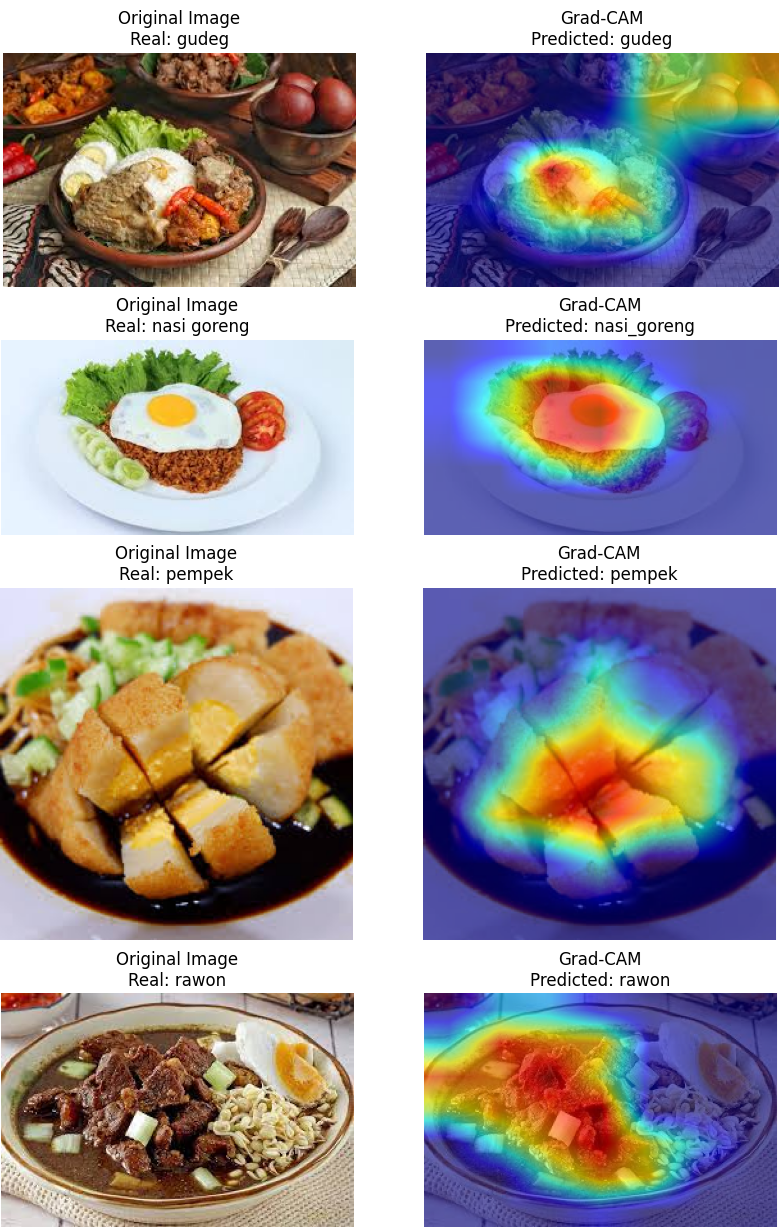
\includegraphics[width=0.9\textwidth, center]{images/grad-cam-2.png}
    \label{fig:grad-cam-2}
\end{afigure}
\clearpage
\begin{afigure}
    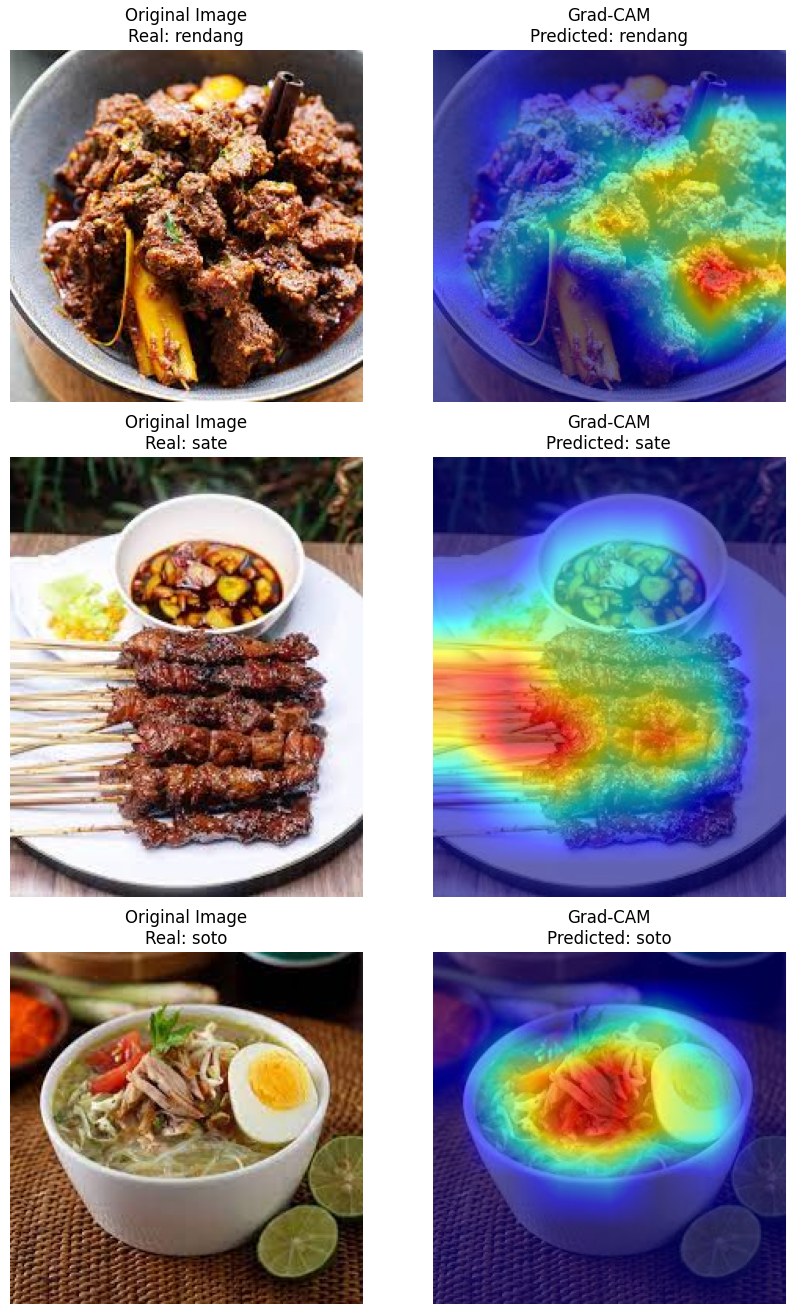
\includegraphics[width=0.9\textwidth, center]{images/grad-cam-3.png}
    \caption{Hasil Visualisasi Grad-CAM Model Google Colab GPU T4}
    \label{fig:grad-cam-3}
\end{afigure}

\clearpage

Pada Gambar 4.9, terlihat bahwa model mampu mengklasifikasikan 9 dari 10 citra dengan tepat. Namun, terdapat satu kelas yang memerlukan perhatian lebih lanjut, yaitu kelas bakso. Dalam visualisasi tersebut, kelas bakso diklasifikasikan sebagai gado-gado. Hal ini menunjukkan bahwa model mengalami kesulitan dalam membedakan antara kedua jenis makanan tersebut.

\subsubsection{Hasil Pengujian Model menggunakan data nutrisi makanan}
Setelah memastikan model memiliki performa yang bagus, selanjutnya dilakukan uji coba menggunakan data nutrisi makanan. Makanan yang berhasil diklasifikasikan kemudian akan ditampilkan informasi nutrisi pada makanan tersebut. Berikut hasil dari uji coba model menggunakan data nutrisi makanan: 
\begin{afigure}
    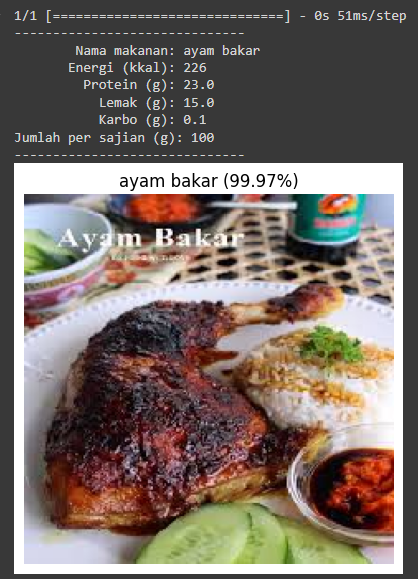
\includegraphics[height=0.55\textheight, width=0.9\textwidth, center]{images/predict-1.png}
    \label{fig:predict-1}
\end{afigure}
\pagebreak
\begin{afigure}
    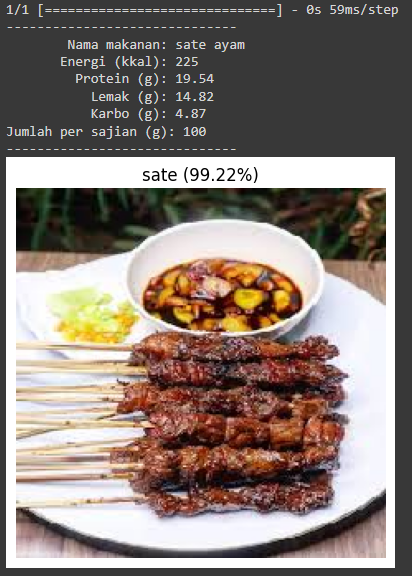
\includegraphics[height=0.55\textheight, width=0.9\textwidth, center]{images/predict-2.png}
    \caption{Hasil Pengujian Model Google Colab GPU T4 menggunakan data nutrisi makanan}
    \label{fig:predict-2}
\end{afigure}

Pada Gambar 4.10 terlihat bahwa model dapat digunakan dan informasi nutrisi dapat ditampilkan dengan baik. Citra juga berhasil diklasifikasikan dengan tepat, citra pertama berhasil diklasifikasikan sebagai ayam bakar dengan \textit{confidence} sebesar 99.97\%, kemudian citra kedua berhasil diklasifikasikan sebagai sate dengan \textit{confidence} sebesar 99.92\%.

\subsection{Hasil Pengujian Model mesin DGX A100 Universitas Gunadarma}
Hasil Pengujian Model mesin DGX A100 Universitas Gunadarma dibagi menjadi 3 bagian, yaitu:
\begin{enumerate}
    \item Hasil Evaluasi Model
    \item Hasil Visualisasi Grad-CAM
    \item Hasil Pengujian Model menggunakan data nutrisi makanan
\end{enumerate}

\subsubsection{Hasil Evaluasi Model}
Tahap pertama pada Evaluasi Model yaitu untuk mengetahui model tersebut termasuk \textit{overfit, good fit} atau \textit{underfit}. Untuk mengetahui hal tersebut, dapat dilakukan dengan membuat visualisasi dari hasil pelatihan model dengan diagram garis. Berikut hasil visualisasi pelatihan model dengan diagram garis:

\begin{afigure}
    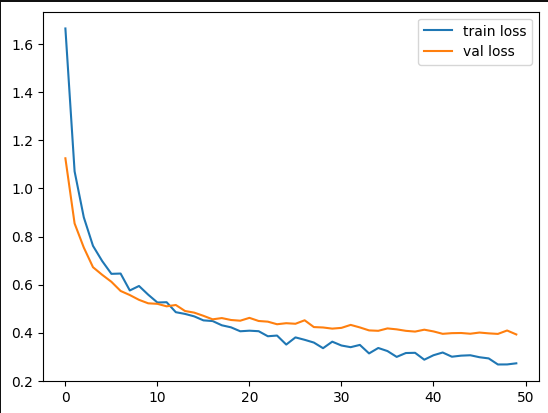
\includegraphics[height=0.4\textheight, width=0.9\textwidth, center]{images/train-loss-dgx.png}
    \label{fig:train-loss-dgx}
\end{afigure}
\pagebreak
\begin{afigure}
    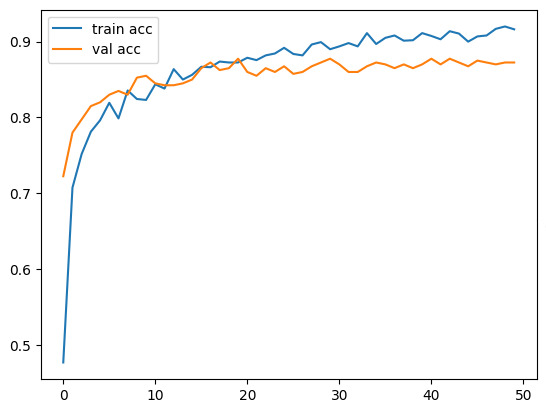
\includegraphics[height=0.4\textheight, width=0.9\textwidth, center]{images/train-acc-dgx.png}
    \caption{Visualisasi Pelatihan Model mesin DGX A100 Universitas Gunadarma}
    \label{fig:train-acc-dgx}
\end{afigure}

Pada Gambar 4.11, terlihat \textit{train loss} dan \textit{val loss} mendekati satu sama lain dan terus menurun hingga datar dari beberapa titik hingga akhir. Kemudian, \textit{train acc} dan \textit{val acc} juga mendekati satu sama lain. Hal ini dapat diartikan bahwa model tersebut termasuk \textit{good fit} dan layak dipakai.

Setelah mengetahui bahwa model layak dipakai, kemudian dilakukan \textit{
Classification Report} untuk mengetahui performa model berdasarkan metriks \textit{precision}, \textit{recall}, dan \textit{F1-Score}. Berikut hasil dari \textit{Classification Report} menggunakan \textit{library} dari sklearn:

\pagebreak

\begin{afigure}
    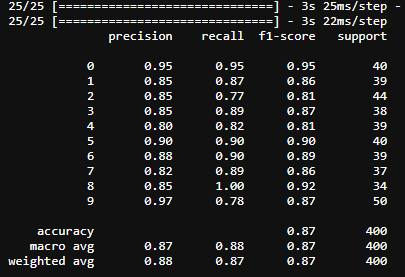
\includegraphics[width=0.9\textwidth, center]{images/classification-report-dgx.png}
    \caption{Hasil Classification Report Model mesin DGX A100 Universitas Gunadarma}
    \label{fig:classification-report-dgx}
\end{afigure}


\begin{itemize}
    \item Accuracy: 0.87, menunjukkan bahwa model ini memiliki tingkat akurasi 88\% di seluruh kelas.
    \item Macro Avg: Rata-rata precision, recall, dan f1-score untuk setiap kelas, tanpa mempertimbangkan jumlah instance di setiap kelas.
    \item Weighted Avg: Rata-rata precision, recall, dan f1-score untuk setiap kelas, dengan mempertimbangkan jumlah instance di setiap kelas.
\end{itemize}

Gambar 4.12 menunjukan bahwa model memiliki performa yang baik di sebagian besar kelas, meskipun ada beberapa kelas yang memiliki nilai \textit{recall} atau \textit{precision} yang lebih rendah. Ada beberapa citra yang salah diklasifikasikan ke kelas lain, contohnya pada kelas 2 (gado-gado) dan kelas 9 (soto).

Setelah dilakukan \textit{Classification Report}, untuk mempermudah evaluasi model dapat menggunakan \textit{confusion matrix}. Berikut visualisasi menggunakan \textit{confusion matrix}:

\begin{afigure}
    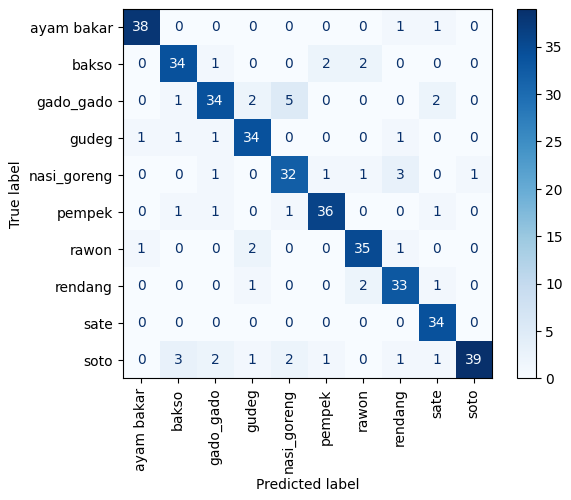
\includegraphics[width=0.9\textwidth, center]{images/confussion-matrix-dgx.png}
    \caption{Visualisasi Confusion Matrix Model mesin DGX A100 Universitas Gunadarma}
    \label{fig:confussion-matrix-dgx}
\end{afigure}

Confusion matrix ini menunjukkan hasil dari model klasifikasi yang telah diuji dengan beberapa kategori makanan Indonesia. Berikut adalah interpretasi dari setiap elemen dalam \textit{confusion matrix} ini:
\begin{itemize}
    \item \textit{True label} (label sebenarnya) berada pada sumbu Y (vertikal).
    \item \textit{Predicted label} (label prediksi) berada pada sumbu X (horizontal).
\end{itemize}

Setiap sel dalam matriks menunjukkan jumlah instance yang diprediksi dalam kategori tertentu. Misalnya, sel pada baris "ayam bakar" dan kolom "ayam bakar" menunjukkan jumlah instance "ayam bakar" yang diprediksi benar oleh model. Berikut adalah beberapa poin penting yang dapat diperhatikan dari \textit{confusion matrix} pada Gambar 4.13:
\begin{itemize}
    \item \textbf{Ayam Bakar}: Dari 40 instance "ayam bakar", 38 diprediksi benar sebagai "ayam bakar", 1 diprediksi sebagai "gudeg", dan 1 diprediksi sebagai "rawon".
    \item \textbf{Bakso}: Dari 40 instance "bakso", 34 diprediksi benar sebagai "bakso", 1 diprediksi sebagai "nasi goreng", 1 diprediksi sebagai "gado-gado", 1 diprediksi sebagai "gudeg", dan 3 diprediksi sebagai "soto".
    \item \textbf{Gado-gado}: Dari 40 instance "gado-gado", 34 diprediksi benar sebagai "gado-gado", 1 diprediksi sebagai "bakso", 1 diprediksi sebagai "gudeg", 1 diprediksi sebagai "nasi goreng", 1 diprediksi sebagai "pempek", dan 2 diprediksi sebagai "soto".
    \item \textbf{Gudeg}: Dari 40 instance "gudeg", 34 diprediksi benar sebagai "gudeg", 2 diprediksi sebagai "gado-gado", 2 diprediksi sebagai "rawon", 1 diprediksi sebagai "rendang", dan 1 diprediksi sebagai "soto".
    \item \textbf{Nasi Goreng}: Dari 40 instance "nasi goreng", 32 diprediksi benar sebagai "nasi goreng", 5 diprediksi sebagai "gado-gado", 1 diprediksi sebagai "pempek", dan 2 diprediksi sebagai "soto".
    \item \textbf{Pempek}: Dari 40 instance "pempek", 36 diprediksi benar sebagai "pempek", 2 diprediksi sebagai "bakso", 1 diprediksi sebagai "nasi goreng", dan 1 diprediksi sebagai "soto".
    \item \textbf{Rawon}: Dari 40 instance "rawon", 35 diprediksi benar sebagai "rawon", 2 diprediksi sebagai "bakso", 1 diprediksi sebagai "nasi goreng", dan 2 diprediksi sebagai "rendang".
    \item \textbf{Rendang}: Dari 40 instance "rendang", 33 diprediksi benar sebagai "rendang", 1 diprediksi sebagai "ayam bakar", 1 diprediksi sebagai "gudeg", 3 diprediksi sebagai "nasi goreng", 1 diprediksi sebagai "rawon", dan 1 diprediksi sebagai "soto".
    \item \textbf{Sate}: Dari 40 instance "sate", 34 diprediksi benar sebagai "sate", 1 diprediksi sebagai "ayam bakar", 2 diprediksi sebagai "gado-gado", 1 diprediksi sebagai "pempek", 1 diprediksi sebagai "rendang", dan 1 diprediksi sebagai "soto".
    \item \textbf{Soto}: Dari 40 instance "soto", 39 diprediksi benar sebagai "soto", 1 diprediksi sebagai "nasi goreng".
\end{itemize}

Secara keseluruhan, model menunjukkan performa yang cukup baik dengan sebagian besar prediksi berada di diagonal utama, yang berarti banyak instance yang diklasifikasikan dengan benar. Namun, ada beberapa kesalahan prediksi yang perlu diperhatikan untuk meningkatkan akurasi model lebih lanjut.

\subsubsection{Hasil Visualisasi Grad-CAM}
Setelah melakukan proses Evaluasi Model, selanjutnya dilakukan proses Visualisasi Grad-CAM. Hal ini dilakukan untuk mengetahui bagaimana model melihat citra dan area mana yang dianggap penting oleh model dalam membuat prediksi. Berikut hasil visualisasi menggunakan Grad-CAM:

\begin{afigure}
    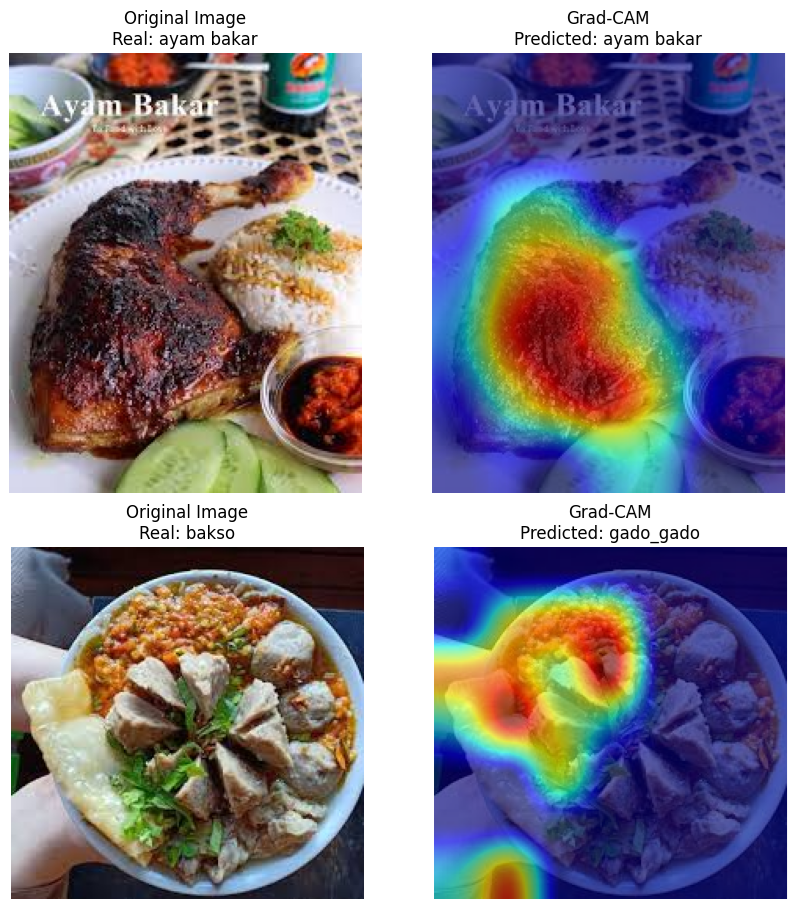
\includegraphics[width=0.9\textwidth, center]{images/grad-cam-1-dgx.png}
    \label{fig:grad-cam-1-dgx}
\end{afigure}
\clearpage
\begin{afigure}
    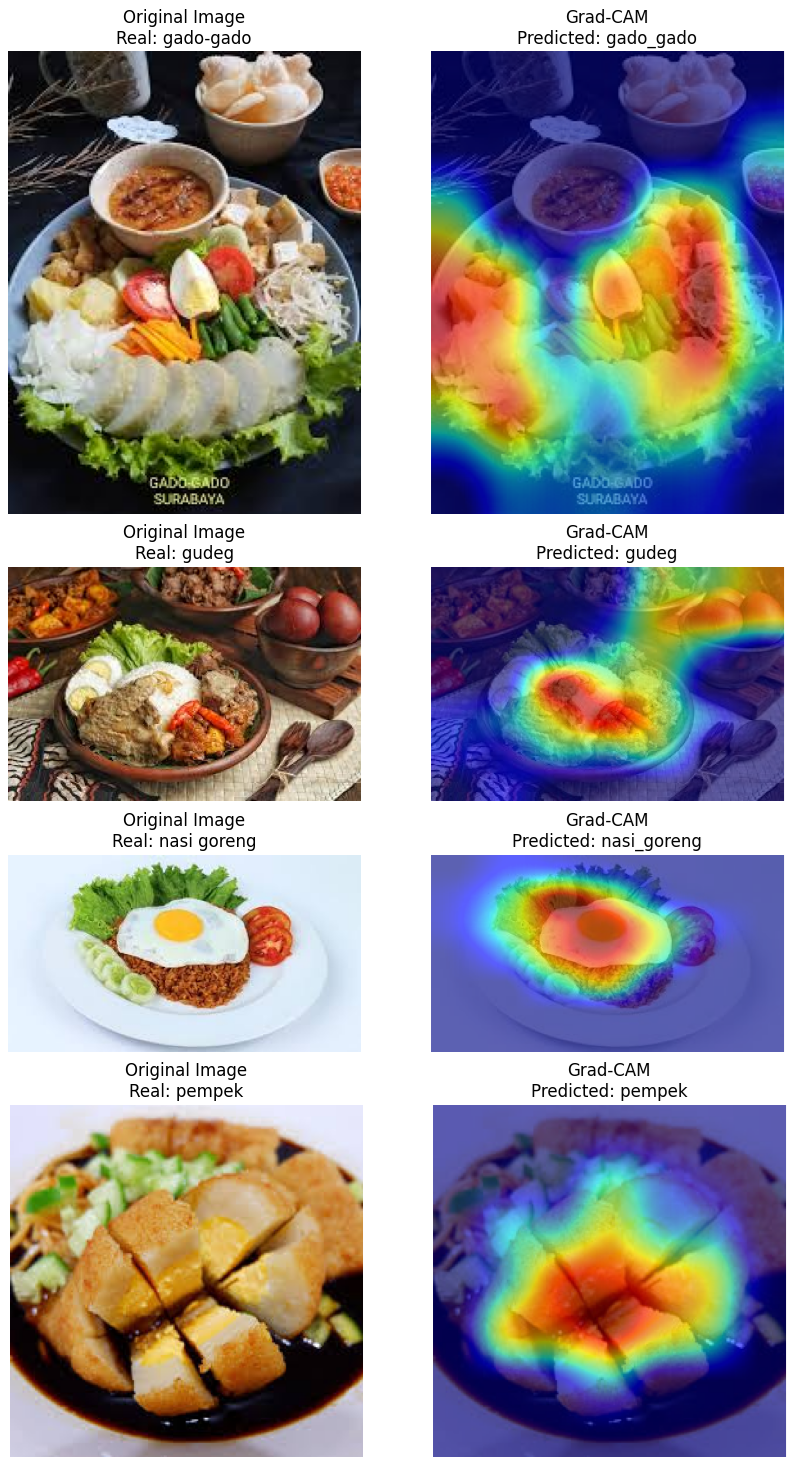
\includegraphics[height=0.9\textheight, width=0.9\textwidth, center]{images/grad-cam-2-dgx.png}
    \label{fig:grad-cam-2-dgx}
\end{afigure}
\clearpage
\begin{afigure}
    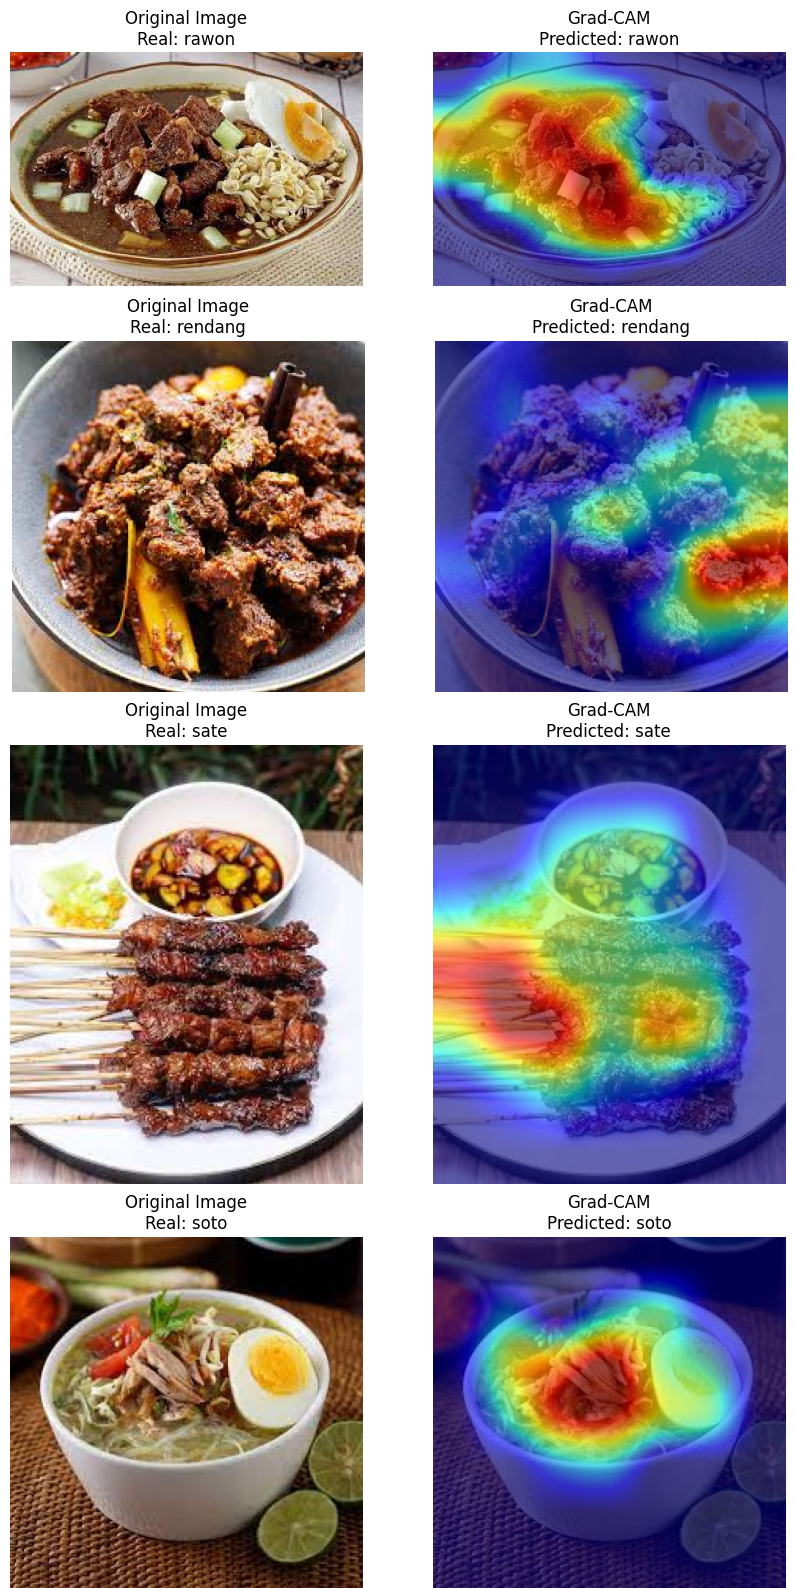
\includegraphics[height=0.9\textheight, width=0.9\textwidth, center]{images/grad-cam-3-dgx.png}
    \caption{Hasil Visualisasi Grad-CAM Model mesin DGX A100 Universitas Gunadarma}
    \label{fig:grad-cam-3-dgx}
\end{afigure}
\clearpage

Pada Gambar 4.14, terlihat bahwa model mampu mengklasifikasikan 9 dari 10 citra dengan tepat. Namun, terdapat satu kelas yang memerlukan perhatian lebih lanjut, yaitu kelas bakso. Dalam visualisasi tersebut, kelas bakso diklasifikasikan sebagai gado-gado. Hal ini menunjukkan bahwa model mengalami kesulitan dalam membedakan antara kedua jenis makanan tersebut.

\subsubsection{Hasil Pengujian Model menggunakan data nutrisi makanan}
Setelah memastikan model memiliki performa yang bagus, selanjutnya dilakukan uji coba menggunakan data nutrisi makanan. Makanan yang berhasil diklasifikasikan kemudian akan ditampilkan informasi nutrisi pada makanan tersebut. Berikut hasil dari uji coba model menggunakan data nutrisi makanan: 
\begin{afigure}
    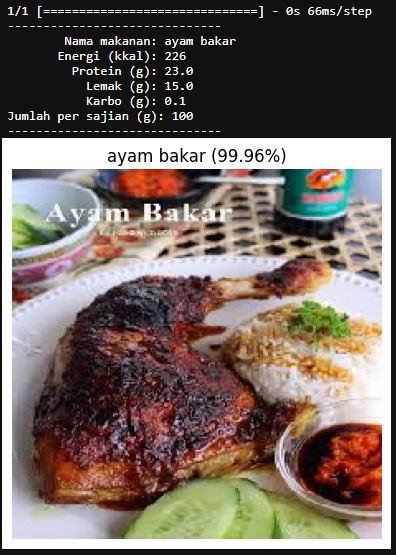
\includegraphics[height=0.55\textheight, width=0.9\textwidth, center]{images/predict-1-dgx.png}
    \label{fig:predict-1-dgx}
\end{afigure}
\pagebreak
\begin{afigure}
    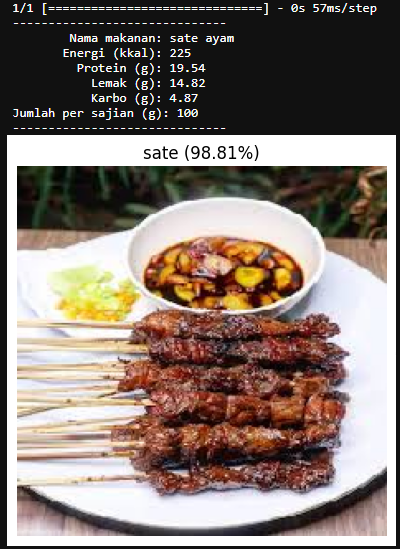
\includegraphics[height=0.55\textheight, width=0.9\textwidth, center]{images/predict-2-dgx.png}
    \caption{Hasil Pengujian Model mesin DGX A100 Universitas Gunadarma menggunakan data nutrisi makanan}
    \label{fig:predict-2-dgx}
\end{afigure}

Pada Gambar 4.15 terlihat bahwa model dapat digunakan dan informasi nutrisi dapat ditampilkan dengan baik. Citra juga berhasil diklasifikasikan dengan tepat, citra pertama berhasil diklasifikasikan sebagai ayam bakar dengan \textit{confidence} sebesar 99.96\%, kemudian citra kedua berhasil diklasifikasikan sebagai sate dengan \textit{confidence} sebesar 98.81\%.



















